\section{Lending Kernel-Owned Buffers}
\label{sec:lending}

The kernel can lend access to a buffer without giving up the right to recycle
its pages. \sys represents the bytes worth keeping as an \emph{object} and
gives the application a handle to it. The handle names data independently of
where it came from. For example, a server can read a range from a block device,
send it to two clients, and release it without reopening the device or reading
the range again.

Two decisions determine how an object can be used. The endpoint defines its unit
of I/O, such as a range of a TCP stream, a UDP datagram, or an aligned block
range. The access mode defines how the application reaches those bytes
(Figure~\ref{fig:modes}). Named mode lends a handle with checked, read-only
access. Mapped mode also lends direct read/write access to a dedicated region
of memory. Either mode can supply a later operation if the destination accepts
the object's length and layout.

\begin{figure}[t]
\centering
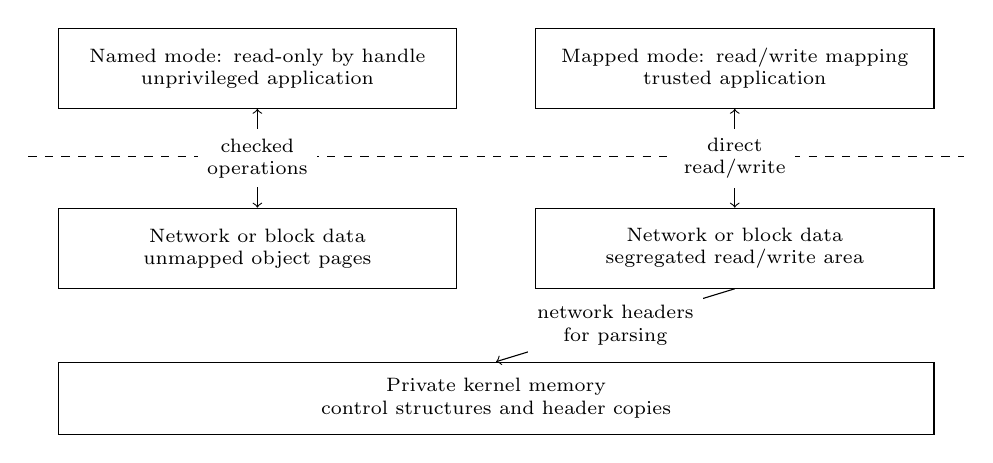
\begin{tikzpicture}[
  every node/.style={font=\scriptsize,align=center},
  accessbox/.style={draw,text width=0.40\columnwidth,minimum height=0.40in,inner sep=3pt}]
\node[accessbox] (namedapp) at (-0.25\columnwidth,0)
  {Named mode: read-only by handle\\unprivileged application};
\node[accessbox] (mappedapp) at (0.25\columnwidth,0)
  {Mapped mode: read/write mapping\\trusted application};
\node[accessbox] (namedkernel) at (-0.25\columnwidth,-0.9in)
  {Network or block data\\unmapped object pages};
\node[accessbox] (mappedkernel) at (0.25\columnwidth,-0.9in)
  {Network or block data\\segregated read/write area};
\node[draw,text width=0.90\columnwidth,minimum height=0.36in,inner sep=3pt]
  (private) at (0,-1.65in)
  {Private kernel memory\\control structures and header copies};
\draw[dashed] (-0.49\columnwidth,-0.44in) -- (0.49\columnwidth,-0.44in);
\draw[<->] (namedapp.south) -- (namedkernel.north)
  node[midway,fill=white] {checked\\operations};
\draw[<->] (mappedapp.south) -- (mappedkernel.north)
  node[midway,fill=white] {direct\\read/write};
\draw[->] (mappedkernel.south) -- (private.north)
  node[midway,fill=white] {network headers\\for parsing};
\end{tikzpicture}
\caption{The dashed line separates the application from the kernel. Both modes give
the application handles. A trusted process can also map the dedicated I/O area.
On network input, the kernel copies headers into private memory before parsing them.}
\label{fig:modes}
\end{figure}

\subsection{One object, three lifetimes}
\label{sec:lending:objects}
\label{sec:named:objects}

Consider the server's last send. The application is finished with the object,
the send may still be queuing bytes to a socket, and TCP may need those bytes
again for retransmission. \sys gives each user a distinct reference.

\begin{enumerate}
\setlength{\itemsep}{2pt}
\item \textbf{The handle} determines whether the application can start another
  operation on the object. Explicit release removes the name. A TCP send
  marked as the last use removes it when the kernel resolves the handle and
  acquires its references, a step we call \emph{admission}.
\item \textbf{The operation} keeps the object's description for as long as it
  needs to locate the bytes. Each admitted TCP send has its own cursor, so a
  slow client can pause without losing another client's place. A block write
  keeps the description through I/O completion.
\item \textbf{The pages} remain live while any consumer holds them. Once TCP
  has queued the send, packets hold their own page references. The kernel can
  drop the ordinary object's description even while TCP retains the data.
  For a mapped receive buffer, the kernel also tracks when the page can safely
  return to the device (\S\ref{sec:mapped:recycle}).
\end{enumerate}

A request submitted on \iouring can still be waiting for admission. Keeping the
handle until completion avoids racing a separate release with that request.
After release, the kernel determines when the pages can be recycled. An
application forwarding objects by handle needs the result of its I/O, but no
additional notification to return the backing memory.

\subsection{Representing and bounding retained data}
\label{sec:lending:cost}

A \emph{store} is the namespace for handles and the unit at which the kernel
limits retained data. It represents each object with a fixed-size \emph{head}
that records its length and state, and a chain of \emph{segments} that locate
its bytes. A segment describes a range within one backing buffer. This lets
the kernel publish a single handle even when a stream range spans several
packets.

At registration the kernel sets aside arrays of heads and segments. Creating
an object takes entries from those arrays, and releasing its description
returns them. This bounds object metadata and avoids allocating it on each
request. Socket queues, buffers for copied data, and mapped I/O regions have
their own memory costs. Sections~\ref{sec:named:memory} and~\ref{sec:mapped:recycle}
explain what holding an object costs in each mode.
